\documentclass[tikz]{standalone}

\begin{document}
	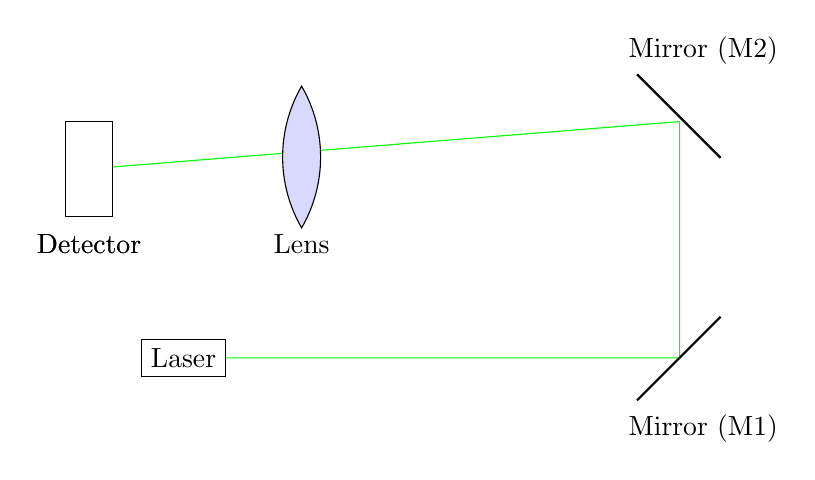
\begin{tikzpicture}[scale=3]
		\pgfmathsetmacro{\lensRadius}{0.6}
		\pgfmathsetmacro{\lensHeight}{.3}
	  	\pgfmathsetmacro{\startAngle}{asin(\lensHeight/\lensRadius)}
	  	\draw[color=green] (0.5, 0) -- ++(2, 0) node(A){} -- ++(0, 1) node(B){} -- ++(-2.5, -0.2);
		\node[draw, fill=white] at (0.4, 0) {Laser};
		\draw[thick] (2.32, -0.18) -- ++(45:0.5);
		\draw[thick] (2.32, 1.2) -- ++(-45:0.5);
		\draw [fill=blue!15]  (0.9,\lensHeight+0.85)
  arc[start angle=180-\startAngle,delta angle=2*\startAngle,radius=\lensRadius]
  arc[start angle=-\startAngle,delta angle=2*\startAngle,radius=\lensRadius]
   -- cycle;
	   \draw[draw=black, fill=white] (-.1, 0.6) rectangle ++(0.2,0.4);
	   \node at (0, 0.48) {Detector};
	   \node at (0.9, 0.48) {Lens};
	   \node at (0, 0.48) {Detector};
	   \node at (2.6, -0.3) {Mirror (M1)};
	   \node at (2.6, +1.3) {Mirror (M2)};
	\end{tikzpicture}
\end{document}
